\section{La Masse des Neutrinos}

Les neutrinos synthétisés dans le plasma chaud de l'Univers primordial sont d'abord maintenus en équilibre avec les photons à travers les réactions $\ell^{-} + \ell^{+} \rightleftharpoons \nu_\ell + \bar{\nu}_\ell$ où $\ell \in \lbrace e, \mu, \tau \rbrace$ est une des 3 saveurs leptoniques\footnote{electronique, muonique et tauique} tant que leur taux ou fréquence de réaction $\Gamma \gg H$ surpasse le taux d'expansion de l'Univers, défini comme la variation logarithmique du facteur d'échelle $a$ dans le temps:

\begin{equation}
H \doteq \frac{1}{a} \frac{d a}{d t} = 100~h~\mathrm{km}~s^{-1}~\mathrm{Mpc}^{-1}
\end{equation}

Lorsque le taux de ces intéractions devient de l'ordre et inférieur à $H$, l'équilibre thermique ne peux plus être maintenu et le neutrino de saveur leptonique associé se découple du plasma. Chacun des neutrinos, $\nu_e, \nu_\mu$ et $\nu_\tau$ se découple lorsque le plasma a une température de plusieurs méga-électron-volts $T_\gamma \sim \mathrm{MeV}$, alors que la masse de chacun des neutrinos est de l'ordre de l'électron-volt $m_\nu \sim \mathrm{eV}$. Chaque neutrino est donc relativiste lorsqu'il se découple du plasma, c'est-à-dire qu'il se comporte comme du rayonnement. En effet, la densité énergétique de la matière relativiste de l'Univers, $\epsilon_r = \rho_r c^2$, est \\
\begin{equation}
\begin{array}{cl}
\epsilon_r & = \epsilon_\gamma + \epsilon_\nu + \epsilon_x \\
\\
 & = \cfrac{8 \pi^2}{15} \cfrac{k_b^4}{h^3 c^3} T_\gamma^4 + \cfrac{7}{8} \cfrac{\pi^2}{15}~N_\mathrm{eff}~T_\nu^4 + \cfrac{7}{8} \cfrac{\pi^2}{15}~\Delta N_\mathrm{eff}~T_x^4\\
\\
 & = \epsilon_\gamma \left[ \cfrac{7}{8} \left( \cfrac{4}{11} \right)^{4/3}~\left( N_\mathrm{eff} + \Delta N_\mathrm{eff} \right) \right]
\end{array}
\end{equation} \\ où les indices $\gamma, \nu, x$ font respectivement référence aux photons de température $T_\gamma$ suivant une loi de corps noir, les $N_\mathrm{eff} \simeq 3$ générations de pairs neutrinos-antineutrinos de température $T_\nu = \left( 4/11 \right)^{1/3} T_\gamma$ et toute autre espèce relativiste couplé aux photons de température $T_x$. La différence de température entre photons et neutrinos est dû au réchauffement du fond diffus lors de l'annihilation électron-positron $e^\pm$ ayant lieu en aval du découplage photon-neutrinos, à $T_\gamma \sim 0.5~\mathrm{MeV}$. En revanche, ce procédé n'a pas lieu instantanément et il s'avère qu'une fraction des neutrinos sont encore couplés au plasma lors de l'annihilation. Si l'on suppose que cet événement est instantané, il faut incorporer ces neutrinos couplés dans la définition du nombre de générations ou saveurs leptoniques des neutrinos
\begin{equation}
N_\mathrm{eff} = 3.046 \pm \Delta N_\mathrm{eff}
\end{equation} avec $\Delta N_\mathrm{eff}$ l'écart par rapport à la valeur prédite par la théorie de $3.046$ à cause d'autres éventuelles espèces relativistes. Puisque les neutrinos sont relativistes lors du découplage, eux aussi voient leur densité énergétique évoluer comme $\epsilon_\nu \propto a^{-4} \propto T_\nu^{4}$. Cet exposant 4 provient du fait que la densité volumique des neutrinos diminue avec le volume, et du fait que leur longueur d'onde associée est elle-aussi diluée avec le facteur d'échelle. Tout comme le fond diffus micro-onde, la théorie du big bang chaud prédit l'existence d'un fond cosmique de neutrinos à $1.9525~\mathrm{K}$. \\

Lorqu'ils furent suggérés comme particules produits par réactions faibles par Enrico Fermi au début du XXe siècle, les neutrinos étaient conçus comme n'ayant pas de masse. Ceci a été infirmé en 1998 après la preuve d'oscillation de leur saveur leptonique au Sudbury National Laboratory dans l'Ontario ainsi qu'au détecteur de la mine Kamioka au Japon \citep{Fukuda1998, Kajita1999, Strumia2006db}. Cette découverte, récompensées par le prix Nobel de physique de l'année 2016 sont une preuve directe qu'au moins un des états de masse a une masse positive, et que les états leptoniques $\left\vert \nu_\ell \right\rangle$ sont une combinaison linéaire des états propres\footnote{état propre au sens de la mécanique quantique, \textit{i.e.} dont son évolution temporelle est déterminé par l'opérateur Hamiltonien.} de masse $\left\vert \nu_i \right\rangle$ ($i \in \lbrace 1, 2, 3 \rbrace$), où les coefficients $U_{\ell i}^\star$ sont donnés par les éléments de la matrice de mélange dite PMNS\footnote{Pontercorvo-Maki-Nakagawa-Sakata}: \\
\begin{equation}
\left\vert \nu_\ell \right\rangle = \sum_{i=1}^{3} U^\star_{\ell i} \left\vert \nu_i \right\rangle
\end{equation} \\ Les sondes cosmologiques sont sensibles à la somme des masses des états propres des neutrinos, $\sum m_\nu = m_1 + m_2 + m_3 \neq m_{\nu_e} + m_{\nu_\mu} + m_{\nu_\tau}$. Dans ce sens, la cosmologie apporte un rôle complémentaire à la physique des particule qui, elle, tente de déterminer la masse des états individuels. À ce jour, la masse des neutrinos reste une question sans réponse, si ce n'est que la somme de leur masse est de l'ordre de l'électron-volt ou inférieur: $\sum m_\nu \sim \mathrm{eV}$. Par ailleurs, les oscillations de saveur leptonique des neutrinos solaires et atmosphériques montrent que les 3 états de masses ne sont pas dégénérés, car en effet \\
\begin{equation}
\left\{
\begin{array}{l}
\delta m^2 = \left( 7.54\pm 0.24 \right) ~\times 10^{-5} ~{\rm eV^2} \\
\\
\Delta m^2 = \left( 2.43\pm 0.06 \right) ~\times 10^{-3} ~{\rm eV^2}
\end{array}
\right.
\end{equation} \\ où $\delta m^2 = m^2_2 - m^2_1$ et $\Delta m^2 = m_3 - (m^2_1 + m^2_2)/2$ d'après la compilation de \cite{Capozzi2013csa}. La somme des masses n'est pas assez contrainte pour distinguer les 2 cas de figure majeurs dans l'ordre ou hiérarchie des états de masse: \\

\begin{itemize}
\item[$\bullet$] \textbf{normal} où 1 état est lourd et les 2 autres sont légers ($\Delta m^2 > 0$), ou \\
\item[$\bullet$] \textbf{inversé} où 1 état est éger et les 2 autres sont lourds ($\Delta m^2 < 0$). \\
\end{itemize} La figure \ref{fig:hierachy} distingue ces 2 ordres par rapport à la configuration dite dégénérée où les différences entre les états de masse sont négligeable par rapport à leur échelle absolue. \\

\begin{figure}
\begin{center}
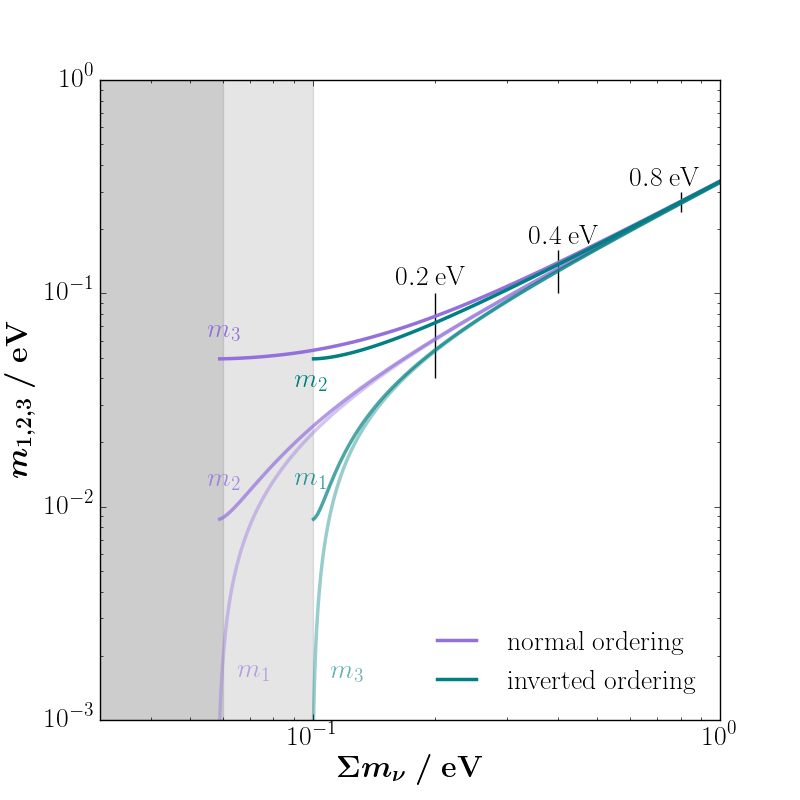
\includegraphics[width=0.75\columnwidth]{Figures/Smnu_mnu.png}
\caption{Valeur des états propres de masse individuels en fonction de la somme des masses $m_1+m_2+m_3$, suivant les deux hiérarchies.}
\label{fig:hierachy}
\end{center}
\end{figure}

Parmi les reliques relativistes supplémentaires, indexées par $x$, sont d'éventuels neutrinos dits \emph{stériles}. Ceux-ci ont une chiralité droitière, à l'inverse des neutrinos ayant une saveur leptonique qui ont une chiralité gauchère. Outre la symétrisation des chiralités, l'existence de neutrinos stériles est motivée théoriquement car elle permettrait aussi d'expliquer les oscillations de saveurs leptoniques, la leptogénèse, et seraient de bons candidats matière noire. Quoi qu'il en soit, la densité énergétique des neutrinos, leptoniques ou stériles, est
\begin{equation}
\label{eq:omnu}
\Omega_\nu h^2 = \frac{m_\nu^\mathrm{eff}}{93.14~\mathrm{eV}}
\end{equation} en unité de densité énergétique critique, ce qui signifie q'un Univers entièrement et uniquement peuplé de neutrinos de $93.14~\mathrm{eV}$ est plat pour un taux d'expansion de $h=1$. La masse effective est, suivant les cas: \\
\begin{equation}
m_\nu^\mathrm{eff} = 
\left\{
\begin{array}{ll}
\sum m_\nu & \text{pour les neutrinos leptoniques} \\
m_{\nu_s} & \text{pour les neutrinos stériles}
\end{array}
\right.
\end{equation} Puisque $sum m_\nu \ll 100~\mathrm{eV}$, les neutrinos leptoniques ne peuvent pas constituer l'entièreté de la matière noire. En revanche, il n'existe aucune contrainte sur la masse des neutrinos stériles $m_{\nu_s}$, et il s'avère que des masses de l'ordre du $\mathrm{keV}$ peuvent être cohérentes avec la matière noire, qui a une densité énergétique de $\Omega_{\mathrm{dm}} \simeq 0.25$ densité critique. \\

\begin{figure}
\begin{center}
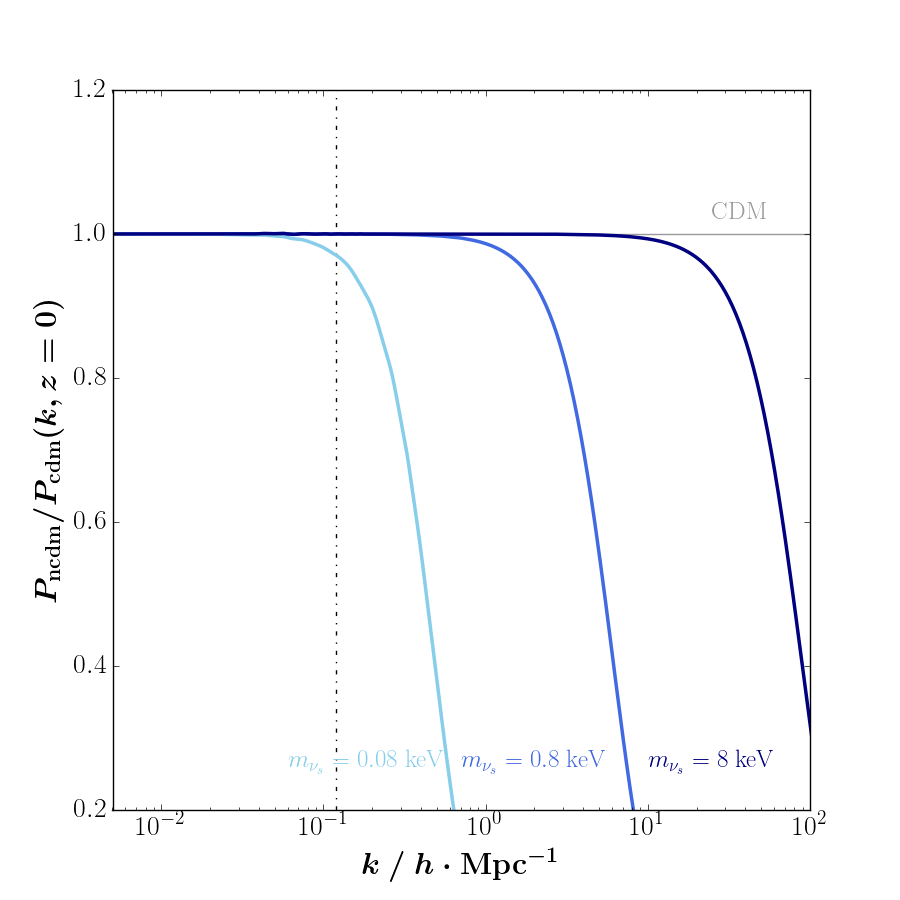
\includegraphics[width=0.55\columnwidth]{Figures/Pk_wdm.png}~%
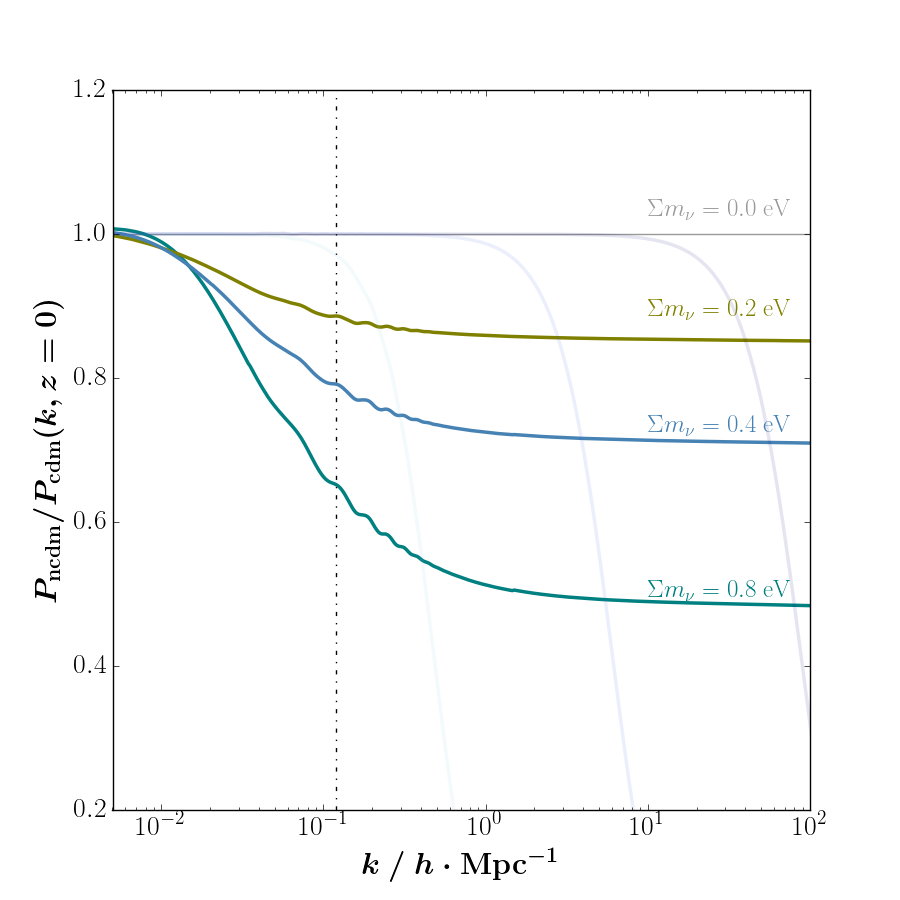
\includegraphics[width=0.55\columnwidth]{Figures/Pk_chdm.png}
\caption{Différence relative du spectre de puissance matière par rapport à un modèle standard (sans neutrinos, en trait gris) à $z=0$.}
\label{fig:pm}
\end{center}
\end{figure}


Tant que les neutrinos se comportent comme du rayonnement, ceux-ci parcourent des distances comparables à leur horizon de particule. Pour des raisons purement cinétique, il ne peuvent pas être contraint dans une région dont les dimensions font la taille de leur horizon. On s'attend donc à témoigner d'un déficit de puissance dans le spectre de puissance de matière aux petites échelles, c'est-à-dire aux grandes valeurs de $k$, la fréquence spatiale, qui se manifeste dans l'encadré de gauche de la figure \ref{fig:pm}. Plus la masse de la particule \footnote{dans ce cas un neutrino stérile constituant l'entièreté de la matière noire} est légère, plus celle-ci parcours des distances élevées et empêche des structures plus larges de s'effondrer par instabilité gravitationnelle. Le spectre de puissance représenté sur cette figure est celui des fluctuations de la matière totale ($=$ matière noire $+$ matière \textit{baryonique}\footnote{c'est-à-dire qui intéragit électromagnétiquement, terme générique qui s'applique à tous les éléments, molécules, gaz, poussières, planètes, étoiles, \textit{etc}.}), définit comme \\
\begin{equation}
P_m(k) = \left\langle \left\vert \sum\limits_{\alpha \in m} \delta_\alpha \right\vert^2 \right\rangle
\end{equation} \\ où $\epsilon = \bar{\epsilon} \left( 1 + \delta \right)$ l'indice $\alpha$ fait référence à la matière noire, la matière baryonique, et les neutrinos une fois non-relativistes. En effet, lorsque la température des photons passe en dessous de la masse d'un état de neutrino, $T_\nu \lesssim m_\nu$, celui-ci devient non-relativiste et se comporte dorénavant comme une composante matière. Sa densité énergétique décroit alors comme $\epsilon_\nu \propto a^{-3}$ et la distance caractéristique qu'il parcours devient fortement inférieur à l'horizon particule. Ils peuvent donc subir l'instabilité gravitationnelle sur les échelles inférieures à cette distance caractéristique, qui dépend de sa masse comme le montre l'encadré de droite de la figure \ref{fig:pm}. Dans ce cas, la grandeur représenté est la spectre de puissance de matière avec des neutrinos leptoniques de masse non nulles et une matière noire dite froide. La somme des masses des neutrinos influence la densité énergétique des neutrinos à travers l'expression \ref{eq:omnu}, et donc la fraction de matière noire dite chaude (c'est-à-dire rapide) par rapport à la froide (quasi-immobile), donnant ainsi l'allure de pallier de puissance constant aux petites échelles. La figure \ref{fig:pm} illustre la signature de la masse des neutrinos sur le spectre de puissance de la matière dans le cadre de la théorie linéaire des perturbations (c'est à dire que $\epsilon_m \ll \bar{\epsilon}_m$). En revanche, les échelles auxquelles ce déficit en puissance se manifeste sont trop basses pour que cette condition s'applique. Pour résoudre le régime linéaire, il faut résoudre l'ensemble des équations gravito-hydrodynamiques à l'aide de simulations numériques, et comparer ces prédictions à la mesure du spectre de puissance de flux transit dans la forêt Ly-$\alpha$.


